% Options for packages loaded elsewhere
\PassOptionsToPackage{unicode}{hyperref}
\PassOptionsToPackage{hyphens}{url}
\PassOptionsToPackage{dvipsnames,svgnames,x11names}{xcolor}
%
\documentclass[
  letterpaper,
  DIV=11,
  numbers=noendperiod]{scrartcl}

\usepackage{amsmath,amssymb}
\usepackage{iftex}
\ifPDFTeX
  \usepackage[T1]{fontenc}
  \usepackage[utf8]{inputenc}
  \usepackage{textcomp} % provide euro and other symbols
\else % if luatex or xetex
  \usepackage{unicode-math}
  \defaultfontfeatures{Scale=MatchLowercase}
  \defaultfontfeatures[\rmfamily]{Ligatures=TeX,Scale=1}
\fi
\usepackage{lmodern}
\ifPDFTeX\else  
    % xetex/luatex font selection
\fi
% Use upquote if available, for straight quotes in verbatim environments
\IfFileExists{upquote.sty}{\usepackage{upquote}}{}
\IfFileExists{microtype.sty}{% use microtype if available
  \usepackage[]{microtype}
  \UseMicrotypeSet[protrusion]{basicmath} % disable protrusion for tt fonts
}{}
\makeatletter
\@ifundefined{KOMAClassName}{% if non-KOMA class
  \IfFileExists{parskip.sty}{%
    \usepackage{parskip}
  }{% else
    \setlength{\parindent}{0pt}
    \setlength{\parskip}{6pt plus 2pt minus 1pt}}
}{% if KOMA class
  \KOMAoptions{parskip=half}}
\makeatother
\usepackage{xcolor}
\setlength{\emergencystretch}{3em} % prevent overfull lines
\setcounter{secnumdepth}{-\maxdimen} % remove section numbering
% Make \paragraph and \subparagraph free-standing
\makeatletter
\ifx\paragraph\undefined\else
  \let\oldparagraph\paragraph
  \renewcommand{\paragraph}{
    \@ifstar
      \xxxParagraphStar
      \xxxParagraphNoStar
  }
  \newcommand{\xxxParagraphStar}[1]{\oldparagraph*{#1}\mbox{}}
  \newcommand{\xxxParagraphNoStar}[1]{\oldparagraph{#1}\mbox{}}
\fi
\ifx\subparagraph\undefined\else
  \let\oldsubparagraph\subparagraph
  \renewcommand{\subparagraph}{
    \@ifstar
      \xxxSubParagraphStar
      \xxxSubParagraphNoStar
  }
  \newcommand{\xxxSubParagraphStar}[1]{\oldsubparagraph*{#1}\mbox{}}
  \newcommand{\xxxSubParagraphNoStar}[1]{\oldsubparagraph{#1}\mbox{}}
\fi
\makeatother

\usepackage{color}
\usepackage{fancyvrb}
\newcommand{\VerbBar}{|}
\newcommand{\VERB}{\Verb[commandchars=\\\{\}]}
\DefineVerbatimEnvironment{Highlighting}{Verbatim}{commandchars=\\\{\}}
% Add ',fontsize=\small' for more characters per line
\usepackage{framed}
\definecolor{shadecolor}{RGB}{241,243,245}
\newenvironment{Shaded}{\begin{snugshade}}{\end{snugshade}}
\newcommand{\AlertTok}[1]{\textcolor[rgb]{0.68,0.00,0.00}{#1}}
\newcommand{\AnnotationTok}[1]{\textcolor[rgb]{0.37,0.37,0.37}{#1}}
\newcommand{\AttributeTok}[1]{\textcolor[rgb]{0.40,0.45,0.13}{#1}}
\newcommand{\BaseNTok}[1]{\textcolor[rgb]{0.68,0.00,0.00}{#1}}
\newcommand{\BuiltInTok}[1]{\textcolor[rgb]{0.00,0.23,0.31}{#1}}
\newcommand{\CharTok}[1]{\textcolor[rgb]{0.13,0.47,0.30}{#1}}
\newcommand{\CommentTok}[1]{\textcolor[rgb]{0.37,0.37,0.37}{#1}}
\newcommand{\CommentVarTok}[1]{\textcolor[rgb]{0.37,0.37,0.37}{\textit{#1}}}
\newcommand{\ConstantTok}[1]{\textcolor[rgb]{0.56,0.35,0.01}{#1}}
\newcommand{\ControlFlowTok}[1]{\textcolor[rgb]{0.00,0.23,0.31}{\textbf{#1}}}
\newcommand{\DataTypeTok}[1]{\textcolor[rgb]{0.68,0.00,0.00}{#1}}
\newcommand{\DecValTok}[1]{\textcolor[rgb]{0.68,0.00,0.00}{#1}}
\newcommand{\DocumentationTok}[1]{\textcolor[rgb]{0.37,0.37,0.37}{\textit{#1}}}
\newcommand{\ErrorTok}[1]{\textcolor[rgb]{0.68,0.00,0.00}{#1}}
\newcommand{\ExtensionTok}[1]{\textcolor[rgb]{0.00,0.23,0.31}{#1}}
\newcommand{\FloatTok}[1]{\textcolor[rgb]{0.68,0.00,0.00}{#1}}
\newcommand{\FunctionTok}[1]{\textcolor[rgb]{0.28,0.35,0.67}{#1}}
\newcommand{\ImportTok}[1]{\textcolor[rgb]{0.00,0.46,0.62}{#1}}
\newcommand{\InformationTok}[1]{\textcolor[rgb]{0.37,0.37,0.37}{#1}}
\newcommand{\KeywordTok}[1]{\textcolor[rgb]{0.00,0.23,0.31}{\textbf{#1}}}
\newcommand{\NormalTok}[1]{\textcolor[rgb]{0.00,0.23,0.31}{#1}}
\newcommand{\OperatorTok}[1]{\textcolor[rgb]{0.37,0.37,0.37}{#1}}
\newcommand{\OtherTok}[1]{\textcolor[rgb]{0.00,0.23,0.31}{#1}}
\newcommand{\PreprocessorTok}[1]{\textcolor[rgb]{0.68,0.00,0.00}{#1}}
\newcommand{\RegionMarkerTok}[1]{\textcolor[rgb]{0.00,0.23,0.31}{#1}}
\newcommand{\SpecialCharTok}[1]{\textcolor[rgb]{0.37,0.37,0.37}{#1}}
\newcommand{\SpecialStringTok}[1]{\textcolor[rgb]{0.13,0.47,0.30}{#1}}
\newcommand{\StringTok}[1]{\textcolor[rgb]{0.13,0.47,0.30}{#1}}
\newcommand{\VariableTok}[1]{\textcolor[rgb]{0.07,0.07,0.07}{#1}}
\newcommand{\VerbatimStringTok}[1]{\textcolor[rgb]{0.13,0.47,0.30}{#1}}
\newcommand{\WarningTok}[1]{\textcolor[rgb]{0.37,0.37,0.37}{\textit{#1}}}

\providecommand{\tightlist}{%
  \setlength{\itemsep}{0pt}\setlength{\parskip}{0pt}}\usepackage{longtable,booktabs,array}
\usepackage{calc} % for calculating minipage widths
% Correct order of tables after \paragraph or \subparagraph
\usepackage{etoolbox}
\makeatletter
\patchcmd\longtable{\par}{\if@noskipsec\mbox{}\fi\par}{}{}
\makeatother
% Allow footnotes in longtable head/foot
\IfFileExists{footnotehyper.sty}{\usepackage{footnotehyper}}{\usepackage{footnote}}
\makesavenoteenv{longtable}
\usepackage{graphicx}
\makeatletter
\def\maxwidth{\ifdim\Gin@nat@width>\linewidth\linewidth\else\Gin@nat@width\fi}
\def\maxheight{\ifdim\Gin@nat@height>\textheight\textheight\else\Gin@nat@height\fi}
\makeatother
% Scale images if necessary, so that they will not overflow the page
% margins by default, and it is still possible to overwrite the defaults
% using explicit options in \includegraphics[width, height, ...]{}
\setkeys{Gin}{width=\maxwidth,height=\maxheight,keepaspectratio}
% Set default figure placement to htbp
\makeatletter
\def\fps@figure{htbp}
\makeatother

\KOMAoption{captions}{tableheading}
\makeatletter
\@ifpackageloaded{caption}{}{\usepackage{caption}}
\AtBeginDocument{%
\ifdefined\contentsname
  \renewcommand*\contentsname{Table of contents}
\else
  \newcommand\contentsname{Table of contents}
\fi
\ifdefined\listfigurename
  \renewcommand*\listfigurename{List of Figures}
\else
  \newcommand\listfigurename{List of Figures}
\fi
\ifdefined\listtablename
  \renewcommand*\listtablename{List of Tables}
\else
  \newcommand\listtablename{List of Tables}
\fi
\ifdefined\figurename
  \renewcommand*\figurename{Figure}
\else
  \newcommand\figurename{Figure}
\fi
\ifdefined\tablename
  \renewcommand*\tablename{Table}
\else
  \newcommand\tablename{Table}
\fi
}
\@ifpackageloaded{float}{}{\usepackage{float}}
\floatstyle{ruled}
\@ifundefined{c@chapter}{\newfloat{codelisting}{h}{lop}}{\newfloat{codelisting}{h}{lop}[chapter]}
\floatname{codelisting}{Listing}
\newcommand*\listoflistings{\listof{codelisting}{List of Listings}}
\makeatother
\makeatletter
\makeatother
\makeatletter
\@ifpackageloaded{caption}{}{\usepackage{caption}}
\@ifpackageloaded{subcaption}{}{\usepackage{subcaption}}
\makeatother

\ifLuaTeX
  \usepackage{selnolig}  % disable illegal ligatures
\fi
\usepackage{bookmark}

\IfFileExists{xurl.sty}{\usepackage{xurl}}{} % add URL line breaks if available
\urlstyle{same} % disable monospaced font for URLs
\hypersetup{
  pdftitle={Visualization (Scales and Guides)},
  pdfauthor={Peter Ganong and Maggie Shi},
  colorlinks=true,
  linkcolor={blue},
  filecolor={Maroon},
  citecolor={Blue},
  urlcolor={Blue},
  pdfcreator={LaTeX via pandoc}}


\title{Visualization (Scales and Guides)}
\author{Peter Ganong and Maggie Shi}
\date{October 21, 2024}

\begin{document}
\maketitle


\section{Intro}\label{intro}

\subsection{roadmap}\label{roadmap}

\begin{itemize}
\tightlist
\item
  define scales and guides
\item
  load and explain dataset
\end{itemize}

(no summary at end because slides are self-contained)

\subsection{scales and guides}\label{scales-and-guides}

``Visual encoding mapping data to visual variables such as position,
size, shape, or color is the beating heart of data visualization.''

Two steps:

\begin{enumerate}
\def\labelenumi{\arabic{enumi}.}
\tightlist
\item
  \emph{scale}: a function that takes a data value as input (the scale
  \emph{domain}) and returns a visual value, such as a pixel position or
  RGB color, as output (the scale \emph{range}).
\item
  \emph{guide}: that allow readers to decode the graphic. Two types:

  \begin{itemize}
  \tightlist
  \item
    \emph{axes} which visualize scales with spatial ranges
  \item
    \emph{legends} which visualize scales with color, size, or shape
    ranges
  \end{itemize}
\end{enumerate}

\subsection{\texorpdfstring{Dataset for this lecture:
\texttt{antibiotics}}{Dataset for this lecture: antibiotics}}\label{dataset-for-this-lecture-antibiotics}

\begin{itemize}
\tightlist
\item
  Each row: a type of bacteria
\item
  Each column: a type of antibiotic
\item
  Each value: \emph{minimum inhibitory concentration (MIC)} the
  concentration of antibiotic (in micrograms per milliliter) required to
  prevent growth in vitro. Lower values means antibiotic is \emph{more
  effective}
\item
  There are two other columns with the genus of the bacteria and the
  response to a lab procedure called ``gram staining''. We will come
  back to these later.
\item
  ``In the fall of 1951, Will Burtin published this graph showing the
  effectiveness of three popular antibiotics on 16 different bacteria,
  measured in terms of minimum inhibitory concentration.''
  \href{http://borgar.net/s/2016/03/will-burtins-antibiotics/}{source}
\end{itemize}

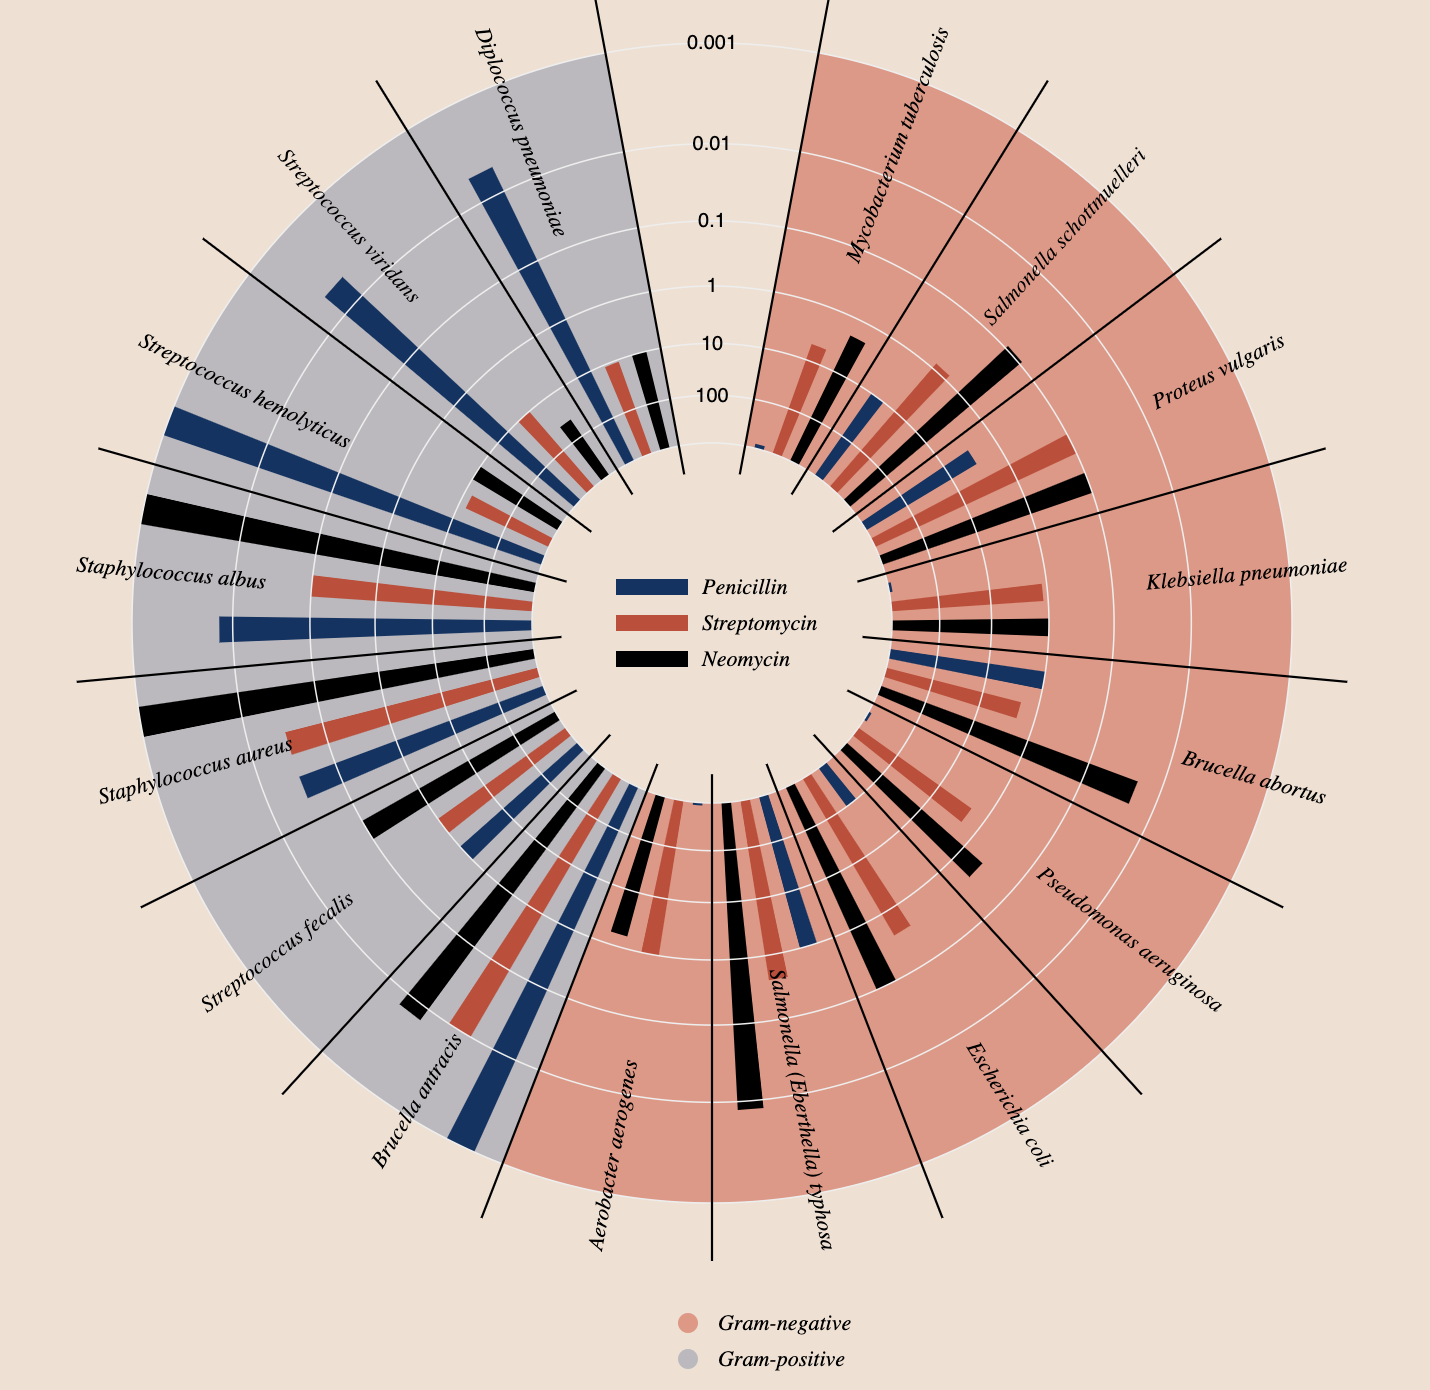
\includegraphics{pictures/burtin.png}

Discussion questions

\begin{itemize}
\tightlist
\item
  headline? (aka the main message)
\item
  sub-messages? (other information one can learn beyond the main
  message)
\end{itemize}

\subsection{Our research questions}\label{our-research-questions}

We will dive deeper into his data with the following research questions:

\begin{enumerate}
\def\labelenumi{\arabic{enumi}.}
\tightlist
\item
  How effective is neomycin against different types of bacteria?
\item
  How does neomycin compare to other antibiotics, such as streptomycin
  and penicillin?
\item
  For which types of bacteria are neomycin and penicillin effective?
\end{enumerate}

\begin{Shaded}
\begin{Highlighting}[]
\ImportTok{import}\NormalTok{ pandas }\ImportTok{as}\NormalTok{ pd}
\ImportTok{import}\NormalTok{ altair }\ImportTok{as}\NormalTok{ alt}
\end{Highlighting}
\end{Shaded}

\begin{Shaded}
\begin{Highlighting}[]
\NormalTok{antibiotics }\OperatorTok{=} \StringTok{\textquotesingle{}https://cdn.jsdelivr.net/npm/vega{-}datasets@1/data/burtin.json\textquotesingle{}}
\NormalTok{pd.read\_json(antibiotics)}
\end{Highlighting}
\end{Shaded}

\begin{Shaded}
\begin{Highlighting}[]
\NormalTok{antibiotics[[}\StringTok{\textquotesingle{}Bacteria\textquotesingle{}}\NormalTok{, }\StringTok{\textquotesingle{}Penicillin\textquotesingle{}}\NormalTok{, }\StringTok{\textquotesingle{}Streptomycin\textquotesingle{}}\NormalTok{, }\StringTok{\textquotesingle{}Neomycin\textquotesingle{}}\NormalTok{]].head()}
\end{Highlighting}
\end{Shaded}

\begin{longtable}[]{@{}lllll@{}}
\toprule\noalign{}
& Bacteria & Penicillin & Streptomycin & Neomycin \\
\midrule\noalign{}
\endhead
\bottomrule\noalign{}
\endlastfoot
0 & Aerobacter aerogenes & 870.000 & 1.00 & 1.600 \\
1 & Bacillus anthracis & 0.001 & 0.01 & 0.007 \\
2 & Brucella abortus & 1.000 & 2.00 & 0.020 \\
3 & Diplococcus pneumoniae & 0.005 & 11.00 & 10.000 \\
4 & Escherichia coli & 100.000 & 0.40 & 0.100 \\
\end{longtable}

Discussion questions:

\begin{itemize}
\tightlist
\item
  are these data ``tidy''?
\item
  if no, how would you tidy them?
\end{itemize}

\section{Configuring Scales and Axes}\label{configuring-scales-and-axes}

\subsection{Configuring Scales and Axes:
roadmap}\label{configuring-scales-and-axes-roadmap}

\begin{itemize}
\tightlist
\item
  manipulate \texttt{alt.Scale()}
\item
  clarify the meaning implied by an axis
\item
  change the length (\texttt{domain}) of an axis
\item
  change grid lines via \texttt{alt.Axis()}
\end{itemize}

\subsection{Plotting Antibiotic Resistance: Adjusting the Scale
Type}\label{plotting-antibiotic-resistance-adjusting-the-scale-type}

Default scale is linear

\begin{Shaded}
\begin{Highlighting}[]
\NormalTok{alt.Chart(antibiotics).mark\_circle().encode(}
\NormalTok{    alt.X(}\StringTok{\textquotesingle{}Neomycin:Q\textquotesingle{}}\NormalTok{)}
\NormalTok{)}
\end{Highlighting}
\end{Shaded}

\begin{verbatim}
alt.Chart(...)
\end{verbatim}

Discussion question: why is this plot hard to read?

\subsection{alt scale I}\label{alt-scale-i}

\begin{Shaded}
\begin{Highlighting}[]
\NormalTok{alt.Chart(antibiotics).mark\_circle().encode(}
\NormalTok{    alt.X(}\StringTok{\textquotesingle{}Neomycin:Q\textquotesingle{}}\NormalTok{,}
\NormalTok{          scale}\OperatorTok{=}\NormalTok{alt.Scale(}\BuiltInTok{type}\OperatorTok{=}\StringTok{\textquotesingle{}sqrt\textquotesingle{}}\NormalTok{))}
\NormalTok{)}
\end{Highlighting}
\end{Shaded}

\begin{verbatim}
alt.Chart(...)
\end{verbatim}

\subsection{alt scale II}\label{alt-scale-ii}

\begin{Shaded}
\begin{Highlighting}[]
\NormalTok{alt.Chart(antibiotics).mark\_circle().encode(}
\NormalTok{    alt.X(}\StringTok{\textquotesingle{}Neomycin:Q\textquotesingle{}}\NormalTok{,}
\NormalTok{          scale}\OperatorTok{=}\NormalTok{alt.Scale(}\BuiltInTok{type}\OperatorTok{=}\StringTok{\textquotesingle{}log\textquotesingle{}}\NormalTok{))}
\NormalTok{)}
\end{Highlighting}
\end{Shaded}

\begin{verbatim}
alt.Chart(...)
\end{verbatim}

Discussion question: what does this plot do well? What is confusing
about it?

\subsection{Styling an Axis}\label{styling-an-axis}

\begin{itemize}
\tightlist
\item
  Lower dosages indicate higher effectiveness. However, many readers
  will expect values that are ``better'' to be ``up and to the right''
  within a chart.
\item
  If we want to cater to this convention set the encoding \texttt{sort}
  property to \texttt{\textquotesingle{}descending\textquotesingle{}}:
\end{itemize}

\begin{Shaded}
\begin{Highlighting}[]
\NormalTok{alt.Chart(antibiotics).mark\_circle().encode(}
\NormalTok{    alt.X(}\StringTok{\textquotesingle{}Neomycin:Q\textquotesingle{}}\NormalTok{,}
\NormalTok{          sort}\OperatorTok{=}\StringTok{\textquotesingle{}descending\textquotesingle{}}\NormalTok{,}
\NormalTok{          scale}\OperatorTok{=}\NormalTok{alt.Scale(}\BuiltInTok{type}\OperatorTok{=}\StringTok{\textquotesingle{}log\textquotesingle{}}\NormalTok{))}
\NormalTok{)}
\end{Highlighting}
\end{Shaded}

\begin{verbatim}
alt.Chart(...)
\end{verbatim}

\subsection{add a clarifying title}\label{add-a-clarifying-title}

\begin{Shaded}
\begin{Highlighting}[]
\NormalTok{alt.Chart(antibiotics).mark\_circle().encode(}
\NormalTok{    alt.X(}\StringTok{\textquotesingle{}Neomycin:Q\textquotesingle{}}\NormalTok{,}
\NormalTok{          sort}\OperatorTok{=}\StringTok{\textquotesingle{}descending\textquotesingle{}}\NormalTok{,}
\NormalTok{          scale}\OperatorTok{=}\NormalTok{alt.Scale(}\BuiltInTok{type}\OperatorTok{=}\StringTok{\textquotesingle{}log\textquotesingle{}}\NormalTok{),}
\NormalTok{          title}\OperatorTok{=}\StringTok{\textquotesingle{}← Less effective {-}{-}{-} Neomycin MIC (μg/ml) {-}{-}{-} more effective →\textquotesingle{}}\NormalTok{)}
\NormalTok{)}
\end{Highlighting}
\end{Shaded}

\begin{verbatim}
alt.Chart(...)
\end{verbatim}

Editorial remark: the textbook suggests a title of ``Neomycin MIC
(μg/ml, reverse log scale)''. This is accurate, but I don't know it
helps the reader that much.

\begin{enumerate}
\def\labelenumi{\arabic{enumi}.}
\tightlist
\item
  The fact that it is a log scale is self-evident. So is the fact that
  it is reversed.
\item
  What the reader really wants to know is which direction is ``good''.
  Just tell them that directly.
\end{enumerate}

\subsection{Comparing Antibiotics: Adjusting Grid Lines, Tick Counts,
and
Sizing}\label{comparing-antibiotics-adjusting-grid-lines-tick-counts-and-sizing}

\emph{How does neomycin compare to streptomycin?}

Question for the class: what does each point repesent?

\begin{Shaded}
\begin{Highlighting}[]
\NormalTok{alt.Chart(antibiotics).mark\_circle().encode(}
\NormalTok{    alt.X(}\StringTok{\textquotesingle{}Neomycin:Q\textquotesingle{}}\NormalTok{,}
\NormalTok{          sort}\OperatorTok{=}\StringTok{\textquotesingle{}descending\textquotesingle{}}\NormalTok{,}
\NormalTok{          scale}\OperatorTok{=}\NormalTok{alt.Scale(}\BuiltInTok{type}\OperatorTok{=}\StringTok{\textquotesingle{}log\textquotesingle{}}\NormalTok{),}
\NormalTok{          title}\OperatorTok{=}\StringTok{\textquotesingle{}← Less effective {-}{-}{-} Neomycin MIC (μg/ml) {-}{-}{-} more effective →\textquotesingle{}}\NormalTok{),}
\NormalTok{    alt.Y(}\StringTok{\textquotesingle{}Streptomycin:Q\textquotesingle{}}\NormalTok{,}
\NormalTok{          sort}\OperatorTok{=}\StringTok{\textquotesingle{}descending\textquotesingle{}}\NormalTok{,}
\NormalTok{          scale}\OperatorTok{=}\NormalTok{alt.Scale(}\BuiltInTok{type}\OperatorTok{=}\StringTok{\textquotesingle{}log\textquotesingle{}}\NormalTok{),}
\NormalTok{          title}\OperatorTok{=}\StringTok{\textquotesingle{}← Less effective {-}{-}{-} Streptomycin MIC (μg/ml) {-}{-}{-} more effective →\textquotesingle{}}\NormalTok{)}
\NormalTok{)}
\end{Highlighting}
\end{Shaded}

\begin{verbatim}
alt.Chart(...)
\end{verbatim}

This plot shows that bacteria responds similarly to these two
antibiotics -- it approximately follows the 45-degree line.

\emph{How does neomycin compare to penicillin?}

\begin{Shaded}
\begin{Highlighting}[]
\NormalTok{alt.Chart(antibiotics).mark\_circle().encode(}
\NormalTok{    alt.X(}\StringTok{\textquotesingle{}Neomycin:Q\textquotesingle{}}\NormalTok{,}
\NormalTok{          sort}\OperatorTok{=}\StringTok{\textquotesingle{}descending\textquotesingle{}}\NormalTok{,}
\NormalTok{          scale}\OperatorTok{=}\NormalTok{alt.Scale(}\BuiltInTok{type}\OperatorTok{=}\StringTok{\textquotesingle{}log\textquotesingle{}}\NormalTok{),}
\NormalTok{          title}\OperatorTok{=}\StringTok{\textquotesingle{}← Less effective {-}{-}{-} Neomycin MIC (μg/ml) {-}{-}{-} more effective →\textquotesingle{}}\NormalTok{),}
\NormalTok{    alt.Y(}\StringTok{\textquotesingle{}Penicillin:Q\textquotesingle{}}\NormalTok{,}
\NormalTok{          sort}\OperatorTok{=}\StringTok{\textquotesingle{}descending\textquotesingle{}}\NormalTok{,}
\NormalTok{          scale}\OperatorTok{=}\NormalTok{alt.Scale(}\BuiltInTok{type}\OperatorTok{=}\StringTok{\textquotesingle{}log\textquotesingle{}}\NormalTok{),}
\NormalTok{          title}\OperatorTok{=}\StringTok{\textquotesingle{}← Less effective {-}{-}{-} Penicillin MIC (μg/ml) {-}{-}{-} more effective →\textquotesingle{}}\NormalTok{)}
\NormalTok{)}
\end{Highlighting}
\end{Shaded}

\begin{verbatim}
alt.Chart(...)
\end{verbatim}

\emph{Now we see a more differentiated response: some bacteria respond
well to neomycin but not penicillin, and vice versa!}

\subsection{\texorpdfstring{fix \texttt{domain}, equalize aspect
ratio}{fix domain, equalize aspect ratio}}\label{fix-domain-equalize-aspect-ratio}

While this plot is useful, we can make it better. The x and y axes use
the same units, but have different extents (the chart width is larger
than the height) and different domains (0.001 to 100 for the x-axis, and
0.001 to 1,000 for the y-axis).

\begin{Shaded}
\begin{Highlighting}[]
\NormalTok{alt.Chart(antibiotics).mark\_circle().encode(}
\NormalTok{    alt.X(}\StringTok{\textquotesingle{}Neomycin:Q\textquotesingle{}}\NormalTok{,}
\NormalTok{          sort}\OperatorTok{=}\StringTok{\textquotesingle{}descending\textquotesingle{}}\NormalTok{,}
\NormalTok{          scale}\OperatorTok{=}\NormalTok{alt.Scale(}\BuiltInTok{type}\OperatorTok{=}\StringTok{\textquotesingle{}log\textquotesingle{}}\NormalTok{, domain}\OperatorTok{=}\NormalTok{[}\FloatTok{0.001}\NormalTok{, }\DecValTok{1000}\NormalTok{]),}
\NormalTok{          title}\OperatorTok{=}\StringTok{\textquotesingle{}← Less effective {-}{-}{-} Neomycin MIC (μg/ml) {-}{-}{-} more effective →\textquotesingle{}}\NormalTok{),}
\NormalTok{    alt.Y(}\StringTok{\textquotesingle{}Penicillin:Q\textquotesingle{}}\NormalTok{,}
\NormalTok{          sort}\OperatorTok{=}\StringTok{\textquotesingle{}descending\textquotesingle{}}\NormalTok{,}
\NormalTok{          scale}\OperatorTok{=}\NormalTok{alt.Scale(}\BuiltInTok{type}\OperatorTok{=}\StringTok{\textquotesingle{}log\textquotesingle{}}\NormalTok{, domain}\OperatorTok{=}\NormalTok{[}\FloatTok{0.001}\NormalTok{, }\DecValTok{1000}\NormalTok{]),}
\NormalTok{          title}\OperatorTok{=}\StringTok{\textquotesingle{}← Less effective {-}{-}{-} Penicillin MIC (μg/ml) {-}{-}{-} more effective →\textquotesingle{}}\NormalTok{)}
\NormalTok{).properties(width}\OperatorTok{=}\DecValTok{250}\NormalTok{, height}\OperatorTok{=}\DecValTok{250}\NormalTok{)}
\end{Highlighting}
\end{Shaded}

\begin{verbatim}
alt.Chart(...)
\end{verbatim}

\subsection{\texorpdfstring{reduce grid clutter with
\texttt{alt.Axis(tickCount=5)}}{reduce grid clutter with alt.Axis(tickCount=5)}}\label{reduce-grid-clutter-with-alt.axistickcount5}

Also set \texttt{mark\_circle(size=80)}

\begin{Shaded}
\begin{Highlighting}[]
\NormalTok{alt.Chart(antibiotics).mark\_circle(size}\OperatorTok{=}\DecValTok{80}\NormalTok{).encode(}
\NormalTok{    alt.X(}\StringTok{\textquotesingle{}Neomycin:Q\textquotesingle{}}\NormalTok{,}
\NormalTok{          sort}\OperatorTok{=}\StringTok{\textquotesingle{}descending\textquotesingle{}}\NormalTok{,}
\NormalTok{          scale}\OperatorTok{=}\NormalTok{alt.Scale(}\BuiltInTok{type}\OperatorTok{=}\StringTok{\textquotesingle{}log\textquotesingle{}}\NormalTok{, domain}\OperatorTok{=}\NormalTok{[}\FloatTok{0.001}\NormalTok{, }\DecValTok{1000}\NormalTok{]),}
\NormalTok{          axis}\OperatorTok{=}\NormalTok{alt.Axis(tickCount}\OperatorTok{=}\DecValTok{5}\NormalTok{),}
\NormalTok{          title}\OperatorTok{=}\StringTok{\textquotesingle{}← Less effective {-}{-}{-} Neomycin MIC (μg/ml) {-}{-}{-} more effective →\textquotesingle{}}\NormalTok{),}
\NormalTok{    alt.Y(}\StringTok{\textquotesingle{}Penicillin:Q\textquotesingle{}}\NormalTok{,}
\NormalTok{          sort}\OperatorTok{=}\StringTok{\textquotesingle{}descending\textquotesingle{}}\NormalTok{,}
\NormalTok{          scale}\OperatorTok{=}\NormalTok{alt.Scale(}\BuiltInTok{type}\OperatorTok{=}\StringTok{\textquotesingle{}log\textquotesingle{}}\NormalTok{, domain}\OperatorTok{=}\NormalTok{[}\FloatTok{0.001}\NormalTok{, }\DecValTok{1000}\NormalTok{]),}
\NormalTok{          axis}\OperatorTok{=}\NormalTok{alt.Axis(tickCount}\OperatorTok{=}\DecValTok{5}\NormalTok{),}
\NormalTok{          title}\OperatorTok{=}\StringTok{\textquotesingle{}← Less effective {-}{-}{-} Penicillin MIC (μg/ml) {-}{-}{-} more effective →\textquotesingle{}}\NormalTok{)}
\NormalTok{).properties(width}\OperatorTok{=}\DecValTok{250}\NormalTok{, height}\OperatorTok{=}\DecValTok{250}\NormalTok{)}
\end{Highlighting}
\end{Shaded}

\begin{verbatim}
alt.Chart(...)
\end{verbatim}

Discussion questions: 1) What questions does this plot answer? 2) What
further questions does this plot raise?

\subsection{Configuring Scales and Axes:
summary}\label{configuring-scales-and-axes-summary}

How to make your axes and grids as informative as possible

\begin{itemize}
\tightlist
\item
  Choose an \texttt{alt.Scale()} that reveals differences between the
  data (in most cases\ldots)
\item
  Axis titles should clarify meaning
\item
  Deliberately choose axis length via \texttt{domain} argument
\item
  Reduce grid clutter via \texttt{alt.Axis()}
\end{itemize}

\section{Configuring Color Legends}\label{configuring-color-legends}

\subsection{Configuring Color Legends: roadmap and
warning}\label{configuring-color-legends-roadmap-and-warning}

\begin{itemize}
\tightlist
\item
  Visualization as a tool for discovery
\item
  \texttt{alt.Color()} in legends

  \begin{itemize}
  \tightlist
  \item
    binary variable
  \item
    text data (every dot is different)
  \item
    groups
  \end{itemize}
\item
  use color to encode quantitative values
\end{itemize}

Remarks:

\begin{itemize}
\tightlist
\item
  This section of the textbook asks you to practice your ``skepticism''
  muscle. What we mean by that is that it is mostly about showing what
  does \emph{not} work. we will follow the textbook, but for many of the
  plots, your first question should not be ``where would I want to use
  this tool?'' but rather ``why is this not a good idea?''
\item
  The official title of this section of lecture is about color legends,
  but the deeper lessons are about how to clean data to uncover and
  communciate structure
\end{itemize}

\subsection{Visualization as a tool for
discovery}\label{visualization-as-a-tool-for-discovery}

\begin{itemize}
\tightlist
\item
  Above we saw that neomycin is more effective for some bacteria, while
  penicillin is more effective for others.
\item
  Is there any systematic answer to what types of bacteria each drug is
  more effective for? This is the kind of question for which data
  visualization shines.
\item
  If we just stared at a table in Excel or Pandas, it might be hard to
  see patterns (and at the very least it would take awhile). Until now,
  almost everything we have seen for data visualization has been about
  \textbf{communication}. Now, we are going to see how data
  visualization can be a tool for \textbf{discovery}.
\end{itemize}

\subsection{Gram staining}\label{gram-staining}

Let's start by looking at one of the other columns in the data frame
(which we have ignored until now).

A tiny bit of science: the reaction of the bacteria to a procedure
called \href{https://en.wikipedia.org/wiki/Gram_stain}{Gram staining} is
described by the nominal field \texttt{Gram\_Staining}. Bacteria that
turn dark blue or violet are Gram-positive. Otherwise, they are
Gram-negative.

\begin{figure}[H]

{\centering \includegraphics{pictures/Gram_stain_01.jpg}

}

\caption{Gram staining example}

\end{figure}%

\begin{Shaded}
\begin{Highlighting}[]
\NormalTok{antibiotics[[}\StringTok{\textquotesingle{}Gram\_Staining\textquotesingle{}}\NormalTok{]].tail()}
\end{Highlighting}
\end{Shaded}

\begin{longtable}[]{@{}ll@{}}
\toprule\noalign{}
& Gram\_Staining \\
\midrule\noalign{}
\endhead
\bottomrule\noalign{}
\endlastfoot
11 & positive \\
12 & positive \\
13 & positive \\
14 & positive \\
15 & positive \\
\end{longtable}

\subsection{alt.Color(`Gram\_Staining:N')}\label{alt.colorgram_stainingn}

Let's encode \texttt{Gram\_Staining} on the \texttt{color} channel as a
nominal data type:

\begin{Shaded}
\begin{Highlighting}[]
\NormalTok{alt.Chart(antibiotics).mark\_circle(size}\OperatorTok{=}\DecValTok{80}\NormalTok{).encode(}
\NormalTok{    alt.X(}\StringTok{\textquotesingle{}Neomycin:Q\textquotesingle{}}\NormalTok{,}
\NormalTok{          sort}\OperatorTok{=}\StringTok{\textquotesingle{}descending\textquotesingle{}}\NormalTok{,}
\NormalTok{          scale}\OperatorTok{=}\NormalTok{alt.Scale(}\BuiltInTok{type}\OperatorTok{=}\StringTok{\textquotesingle{}log\textquotesingle{}}\NormalTok{, domain}\OperatorTok{=}\NormalTok{[}\FloatTok{0.001}\NormalTok{, }\DecValTok{1000}\NormalTok{]),}
\NormalTok{          axis}\OperatorTok{=}\NormalTok{alt.Axis(tickCount}\OperatorTok{=}\DecValTok{5}\NormalTok{),}
\NormalTok{          title}\OperatorTok{=}\StringTok{\textquotesingle{}← Less effective {-}{-}{-} Neomycin MIC (μg/ml) {-}{-}{-} more effective →\textquotesingle{}}\NormalTok{),}
\NormalTok{    alt.Y(}\StringTok{\textquotesingle{}Penicillin:Q\textquotesingle{}}\NormalTok{,}
\NormalTok{          sort}\OperatorTok{=}\StringTok{\textquotesingle{}descending\textquotesingle{}}\NormalTok{,}
\NormalTok{          scale}\OperatorTok{=}\NormalTok{alt.Scale(}\BuiltInTok{type}\OperatorTok{=}\StringTok{\textquotesingle{}log\textquotesingle{}}\NormalTok{, domain}\OperatorTok{=}\NormalTok{[}\FloatTok{0.001}\NormalTok{, }\DecValTok{1000}\NormalTok{]),}
\NormalTok{          axis}\OperatorTok{=}\NormalTok{alt.Axis(tickCount}\OperatorTok{=}\DecValTok{5}\NormalTok{),}
\NormalTok{          title}\OperatorTok{=}\StringTok{\textquotesingle{}← Less effective {-}{-}{-} Penicillin MIC (μg/ml) {-}{-}{-} more effective →\textquotesingle{}}\NormalTok{),}
\NormalTok{    alt.Color(}\StringTok{\textquotesingle{}Gram\_Staining:N\textquotesingle{}}\NormalTok{)}
\NormalTok{).properties(width}\OperatorTok{=}\DecValTok{250}\NormalTok{, height}\OperatorTok{=}\DecValTok{250}\NormalTok{)}
\end{Highlighting}
\end{Shaded}

\begin{verbatim}
alt.Chart(...)
\end{verbatim}

We can see that Gram-positive bacteria seem most susceptible to
penicillin, whereas neomycin is more effective for Gram-negative
bacteria!

\subsection{Sometimes helpful trick: choose colors with external
meaning}\label{sometimes-helpful-trick-choose-colors-with-external-meaning}

However, we might wish to customize the colors used. In this case, we
might want to use the colors that come out in lab when you do gram
staining. Let's use those colors by specifying an explicit scale mapping
from the data \texttt{domain} to the color \texttt{range}:

\begin{Shaded}
\begin{Highlighting}[]
\NormalTok{alt.Chart(antibiotics).mark\_circle(size}\OperatorTok{=}\DecValTok{80}\NormalTok{).encode(}
\NormalTok{    alt.X(}\StringTok{\textquotesingle{}Neomycin:Q\textquotesingle{}}\NormalTok{,}
\NormalTok{          sort}\OperatorTok{=}\StringTok{\textquotesingle{}descending\textquotesingle{}}\NormalTok{,}
\NormalTok{          scale}\OperatorTok{=}\NormalTok{alt.Scale(}\BuiltInTok{type}\OperatorTok{=}\StringTok{\textquotesingle{}log\textquotesingle{}}\NormalTok{, domain}\OperatorTok{=}\NormalTok{[}\FloatTok{0.001}\NormalTok{, }\DecValTok{1000}\NormalTok{]),}
\NormalTok{          axis}\OperatorTok{=}\NormalTok{alt.Axis(tickCount}\OperatorTok{=}\DecValTok{5}\NormalTok{),}
\NormalTok{          title}\OperatorTok{=}\StringTok{\textquotesingle{}← Less effective {-}{-}{-} Neomycin MIC (μg/ml) {-}{-}{-} more effective →\textquotesingle{}}\NormalTok{),}
\NormalTok{    alt.Y(}\StringTok{\textquotesingle{}Penicillin:Q\textquotesingle{}}\NormalTok{,}
\NormalTok{          sort}\OperatorTok{=}\StringTok{\textquotesingle{}descending\textquotesingle{}}\NormalTok{,}
\NormalTok{          scale}\OperatorTok{=}\NormalTok{alt.Scale(}\BuiltInTok{type}\OperatorTok{=}\StringTok{\textquotesingle{}log\textquotesingle{}}\NormalTok{, domain}\OperatorTok{=}\NormalTok{[}\FloatTok{0.001}\NormalTok{, }\DecValTok{1000}\NormalTok{]),}
\NormalTok{          axis}\OperatorTok{=}\NormalTok{alt.Axis(tickCount}\OperatorTok{=}\DecValTok{5}\NormalTok{),}
\NormalTok{          title}\OperatorTok{=}\StringTok{\textquotesingle{}← Less effective {-}{-}{-} Penicillin MIC (μg/ml) {-}{-}{-} more effective →\textquotesingle{}}\NormalTok{),}
\NormalTok{    alt.Color(}\StringTok{\textquotesingle{}Gram\_Staining:N\textquotesingle{}}\NormalTok{,}
\NormalTok{          scale}\OperatorTok{=}\NormalTok{alt.Scale(domain}\OperatorTok{=}\NormalTok{[}\StringTok{\textquotesingle{}negative\textquotesingle{}}\NormalTok{, }\StringTok{\textquotesingle{}positive\textquotesingle{}}\NormalTok{], }\BuiltInTok{range}\OperatorTok{=}\NormalTok{[}\StringTok{\textquotesingle{}hotpink\textquotesingle{}}\NormalTok{, }\StringTok{\textquotesingle{}purple\textquotesingle{}}\NormalTok{])}
\NormalTok{    )}
\NormalTok{).properties(width}\OperatorTok{=}\DecValTok{250}\NormalTok{, height}\OperatorTok{=}\DecValTok{250}\NormalTok{)}
\end{Highlighting}
\end{Shaded}

\begin{verbatim}
alt.Chart(...)
\end{verbatim}

\subsection{Color by Species I}\label{color-by-species-i}

\begin{Shaded}
\begin{Highlighting}[]
\NormalTok{alt.Chart(antibiotics).mark\_circle(size}\OperatorTok{=}\DecValTok{80}\NormalTok{).encode(}
\NormalTok{    alt.X(}\StringTok{\textquotesingle{}Neomycin:Q\textquotesingle{}}\NormalTok{,}
\NormalTok{          sort}\OperatorTok{=}\StringTok{\textquotesingle{}descending\textquotesingle{}}\NormalTok{,}
\NormalTok{          scale}\OperatorTok{=}\NormalTok{alt.Scale(}\BuiltInTok{type}\OperatorTok{=}\StringTok{\textquotesingle{}log\textquotesingle{}}\NormalTok{, domain}\OperatorTok{=}\NormalTok{[}\FloatTok{0.001}\NormalTok{, }\DecValTok{1000}\NormalTok{]),}
\NormalTok{          axis}\OperatorTok{=}\NormalTok{alt.Axis(tickCount}\OperatorTok{=}\DecValTok{5}\NormalTok{),}
\NormalTok{          title}\OperatorTok{=}\StringTok{\textquotesingle{}← Less effective {-}{-}{-} Neomycin MIC (μg/ml) {-}{-}{-} more effective →\textquotesingle{}}\NormalTok{),}
\NormalTok{    alt.Y(}\StringTok{\textquotesingle{}Penicillin:Q\textquotesingle{}}\NormalTok{,}
\NormalTok{          sort}\OperatorTok{=}\StringTok{\textquotesingle{}descending\textquotesingle{}}\NormalTok{,}
\NormalTok{          scale}\OperatorTok{=}\NormalTok{alt.Scale(}\BuiltInTok{type}\OperatorTok{=}\StringTok{\textquotesingle{}log\textquotesingle{}}\NormalTok{, domain}\OperatorTok{=}\NormalTok{[}\FloatTok{0.001}\NormalTok{, }\DecValTok{1000}\NormalTok{]),}
\NormalTok{          axis}\OperatorTok{=}\NormalTok{alt.Axis(tickCount}\OperatorTok{=}\DecValTok{5}\NormalTok{),}
\NormalTok{          title}\OperatorTok{=}\StringTok{\textquotesingle{}← Less effective {-}{-}{-} Penicillin MIC (μg/ml) {-}{-}{-} more effective →\textquotesingle{}}\NormalTok{),}
\NormalTok{    alt.Color(}\StringTok{\textquotesingle{}Bacteria:N\textquotesingle{}}\NormalTok{)}
\NormalTok{).properties(width}\OperatorTok{=}\DecValTok{250}\NormalTok{, height}\OperatorTok{=}\DecValTok{250}\NormalTok{)}
\end{Highlighting}
\end{Shaded}

\begin{verbatim}
alt.Chart(...)
\end{verbatim}

Discussion question: what's wrong with this plot?

\subsection{Color by Species II}\label{color-by-species-ii}

Use \texttt{tableau20} so we have 20 colors instead of 10

\begin{Shaded}
\begin{Highlighting}[]
\NormalTok{alt.Chart(antibiotics).mark\_circle(size}\OperatorTok{=}\DecValTok{80}\NormalTok{).encode(}
\NormalTok{    alt.X(}\StringTok{\textquotesingle{}Neomycin:Q\textquotesingle{}}\NormalTok{,}
\NormalTok{          sort}\OperatorTok{=}\StringTok{\textquotesingle{}descending\textquotesingle{}}\NormalTok{,}
\NormalTok{          scale}\OperatorTok{=}\NormalTok{alt.Scale(}\BuiltInTok{type}\OperatorTok{=}\StringTok{\textquotesingle{}log\textquotesingle{}}\NormalTok{, domain}\OperatorTok{=}\NormalTok{[}\FloatTok{0.001}\NormalTok{, }\DecValTok{1000}\NormalTok{]),}
\NormalTok{          axis}\OperatorTok{=}\NormalTok{alt.Axis(tickCount}\OperatorTok{=}\DecValTok{5}\NormalTok{),}
\NormalTok{          title}\OperatorTok{=}\StringTok{\textquotesingle{}← Less effective {-}{-}{-} Neomycin MIC (μg/ml) {-}{-}{-} more effective →\textquotesingle{}}\NormalTok{),}
\NormalTok{    alt.Y(}\StringTok{\textquotesingle{}Penicillin:Q\textquotesingle{}}\NormalTok{,}
\NormalTok{          sort}\OperatorTok{=}\StringTok{\textquotesingle{}descending\textquotesingle{}}\NormalTok{,}
\NormalTok{          scale}\OperatorTok{=}\NormalTok{alt.Scale(}\BuiltInTok{type}\OperatorTok{=}\StringTok{\textquotesingle{}log\textquotesingle{}}\NormalTok{, domain}\OperatorTok{=}\NormalTok{[}\FloatTok{0.001}\NormalTok{, }\DecValTok{1000}\NormalTok{]),}
\NormalTok{          axis}\OperatorTok{=}\NormalTok{alt.Axis(tickCount}\OperatorTok{=}\DecValTok{5}\NormalTok{),}
\NormalTok{          title}\OperatorTok{=}\StringTok{\textquotesingle{}← Less effective {-}{-}{-} Penicillin MIC (μg/ml) {-}{-}{-} more effective →\textquotesingle{}}\NormalTok{),}
\NormalTok{    alt.Color(}\StringTok{\textquotesingle{}Bacteria:N\textquotesingle{}}\NormalTok{,}
\NormalTok{          scale}\OperatorTok{=}\NormalTok{alt.Scale(scheme}\OperatorTok{=}\StringTok{\textquotesingle{}tableau20\textquotesingle{}}\NormalTok{))}
\NormalTok{).properties(width}\OperatorTok{=}\DecValTok{250}\NormalTok{, height}\OperatorTok{=}\DecValTok{250}\NormalTok{)}
\end{Highlighting}
\end{Shaded}

\begin{verbatim}
alt.Chart(...)
\end{verbatim}

Problem with this plot: bacteria that are similar (all in the ``staph''
family) have very different colors

\subsection{\texorpdfstring{Color by Species III -- color as
\texttt{O}}{Color by Species III -- color as O}}\label{color-by-species-iii-color-as-o}

\begin{Shaded}
\begin{Highlighting}[]
\NormalTok{alt.Chart(antibiotics).mark\_circle(size}\OperatorTok{=}\DecValTok{80}\NormalTok{).encode(}
\NormalTok{    alt.X(}\StringTok{\textquotesingle{}Neomycin:Q\textquotesingle{}}\NormalTok{,}
\NormalTok{          sort}\OperatorTok{=}\StringTok{\textquotesingle{}descending\textquotesingle{}}\NormalTok{,}
\NormalTok{          scale}\OperatorTok{=}\NormalTok{alt.Scale(}\BuiltInTok{type}\OperatorTok{=}\StringTok{\textquotesingle{}log\textquotesingle{}}\NormalTok{, domain}\OperatorTok{=}\NormalTok{[}\FloatTok{0.001}\NormalTok{, }\DecValTok{1000}\NormalTok{]),}
\NormalTok{          axis}\OperatorTok{=}\NormalTok{alt.Axis(tickCount}\OperatorTok{=}\DecValTok{5}\NormalTok{),}
\NormalTok{          title}\OperatorTok{=}\StringTok{\textquotesingle{}← Less effective {-}{-}{-} Neomycin MIC (μg/ml) {-}{-}{-} more effective →\textquotesingle{}}\NormalTok{),}
\NormalTok{    alt.Y(}\StringTok{\textquotesingle{}Penicillin:Q\textquotesingle{}}\NormalTok{,}
\NormalTok{          sort}\OperatorTok{=}\StringTok{\textquotesingle{}descending\textquotesingle{}}\NormalTok{,}
\NormalTok{          scale}\OperatorTok{=}\NormalTok{alt.Scale(}\BuiltInTok{type}\OperatorTok{=}\StringTok{\textquotesingle{}log\textquotesingle{}}\NormalTok{, domain}\OperatorTok{=}\NormalTok{[}\FloatTok{0.001}\NormalTok{, }\DecValTok{1000}\NormalTok{]),}
\NormalTok{          axis}\OperatorTok{=}\NormalTok{alt.Axis(tickCount}\OperatorTok{=}\DecValTok{5}\NormalTok{),}
\NormalTok{          title}\OperatorTok{=}\StringTok{\textquotesingle{}← Less effective {-}{-}{-} Penicillin MIC (μg/ml) {-}{-}{-} more effective →\textquotesingle{}}\NormalTok{),}
\NormalTok{    alt.Color(}\StringTok{\textquotesingle{}Bacteria:O\textquotesingle{}}\NormalTok{)}
\NormalTok{).properties(width}\OperatorTok{=}\DecValTok{250}\NormalTok{, height}\OperatorTok{=}\DecValTok{250}\NormalTok{)}
\end{Highlighting}
\end{Shaded}

\begin{verbatim}
alt.Chart(...)
\end{verbatim}

Problems with this plot:

\begin{enumerate}
\def\labelenumi{\arabic{enumi}.}
\tightlist
\item
  the blue shades are hard to distinguish from one another.
\item
  although it is nice to assign similar colors to bacteria in the same
  family, this legend also assigns similar colors to bacteria that are
  not in the same family
\end{enumerate}

A partial solution to (1) is to use a different color scheme

\subsection{\texorpdfstring{Color by Species IV -- use
\texttt{viridis}}{Color by Species IV -- use viridis}}\label{color-by-species-iv-use-viridis}

This scheme increases both hue and luminance

\begin{Shaded}
\begin{Highlighting}[]
\NormalTok{alt.Chart(antibiotics).mark\_circle(size}\OperatorTok{=}\DecValTok{80}\NormalTok{).encode(}
\NormalTok{    alt.X(}\StringTok{\textquotesingle{}Neomycin:Q\textquotesingle{}}\NormalTok{,}
\NormalTok{          sort}\OperatorTok{=}\StringTok{\textquotesingle{}descending\textquotesingle{}}\NormalTok{,}
\NormalTok{          scale}\OperatorTok{=}\NormalTok{alt.Scale(}\BuiltInTok{type}\OperatorTok{=}\StringTok{\textquotesingle{}log\textquotesingle{}}\NormalTok{, domain}\OperatorTok{=}\NormalTok{[}\FloatTok{0.001}\NormalTok{, }\DecValTok{1000}\NormalTok{]),}
\NormalTok{          axis}\OperatorTok{=}\NormalTok{alt.Axis(tickCount}\OperatorTok{=}\DecValTok{5}\NormalTok{),}
\NormalTok{          title}\OperatorTok{=}\StringTok{\textquotesingle{}← Less effective {-}{-}{-} Neomycin MIC (μg/ml) {-}{-}{-} more effective →\textquotesingle{}}\NormalTok{),}
\NormalTok{    alt.Y(}\StringTok{\textquotesingle{}Penicillin:Q\textquotesingle{}}\NormalTok{,}
\NormalTok{          sort}\OperatorTok{=}\StringTok{\textquotesingle{}descending\textquotesingle{}}\NormalTok{,}
\NormalTok{          scale}\OperatorTok{=}\NormalTok{alt.Scale(}\BuiltInTok{type}\OperatorTok{=}\StringTok{\textquotesingle{}log\textquotesingle{}}\NormalTok{, domain}\OperatorTok{=}\NormalTok{[}\FloatTok{0.001}\NormalTok{, }\DecValTok{1000}\NormalTok{]),}
\NormalTok{          axis}\OperatorTok{=}\NormalTok{alt.Axis(tickCount}\OperatorTok{=}\DecValTok{5}\NormalTok{),}
\NormalTok{          title}\OperatorTok{=}\StringTok{\textquotesingle{}← Less effective {-}{-}{-} Penicillin MIC (μg/ml) {-}{-}{-} more effective →\textquotesingle{}}\NormalTok{),}
\NormalTok{    alt.Color(}\StringTok{\textquotesingle{}Bacteria:O\textquotesingle{}}\NormalTok{,}
\NormalTok{          scale}\OperatorTok{=}\NormalTok{alt.Scale(scheme}\OperatorTok{=}\StringTok{\textquotesingle{}viridis\textquotesingle{}}\NormalTok{))}
\NormalTok{).properties(width}\OperatorTok{=}\DecValTok{250}\NormalTok{, height}\OperatorTok{=}\DecValTok{250}\NormalTok{)}
\end{Highlighting}
\end{Shaded}

\begin{verbatim}
alt.Chart(...)
\end{verbatim}

\subsection{Discussion questions}\label{discussion-questions}

Examples III and IV are jury-rigged to work nicely. They work because

\begin{itemize}
\tightlist
\item
  legend is ordered alphabetically
\item
  bacteria family is at the beginning of the name of each strain.
\end{itemize}

Suppose instead that the family was instead at the \emph{end} of the
name

\begin{longtable}[]{@{}l@{}}
\toprule\noalign{}
bacteria name \\
\midrule\noalign{}
\endhead
\bottomrule\noalign{}
\endlastfoot
Viridans, streptococcus \\
Hemolycticus, Streptococcus \\
\end{longtable}

Let's troubleshoot in real-time. How would you get the color scheme to
align with family? There's more than one good way to do this.

\subsection{Text Labels by Species}\label{text-labels-by-species}

A more clear way to handle this is to use \texttt{mark\_text()} to
explicitly label each dot. However, that comes at the cost of adding a
lot of chart clutter.

\begin{Shaded}
\begin{Highlighting}[]
\NormalTok{base }\OperatorTok{=}\NormalTok{ alt.Chart(antibiotics).mark\_circle(size}\OperatorTok{=}\DecValTok{80}\NormalTok{).encode(}
\NormalTok{    alt.X(}\StringTok{\textquotesingle{}Penicillin:Q\textquotesingle{}}\NormalTok{,}
\NormalTok{          sort}\OperatorTok{=}\StringTok{\textquotesingle{}descending\textquotesingle{}}\NormalTok{,}
\NormalTok{          scale}\OperatorTok{=}\NormalTok{alt.Scale(}\BuiltInTok{type}\OperatorTok{=}\StringTok{\textquotesingle{}log\textquotesingle{}}\NormalTok{, domain}\OperatorTok{=}\NormalTok{[}\FloatTok{0.001}\NormalTok{, }\DecValTok{1000}\NormalTok{]),}
\NormalTok{          axis}\OperatorTok{=}\NormalTok{alt.Axis(tickCount}\OperatorTok{=}\DecValTok{5}\NormalTok{),}
\NormalTok{          title}\OperatorTok{=}\StringTok{\textquotesingle{}← Less effective {-}{-}{-} Penicillin MIC (μg/ml) {-}{-}{-} more effective →\textquotesingle{}}\NormalTok{),}
\NormalTok{    alt.Y(}\StringTok{\textquotesingle{}Streptomycin:Q\textquotesingle{}}\NormalTok{,}
\NormalTok{          scale}\OperatorTok{=}\NormalTok{alt.Scale(}\BuiltInTok{type}\OperatorTok{=}\StringTok{\textquotesingle{}log\textquotesingle{}}\NormalTok{, domain}\OperatorTok{=}\NormalTok{[}\FloatTok{0.001}\NormalTok{, }\DecValTok{1000}\NormalTok{]),}
\NormalTok{          axis}\OperatorTok{=}\NormalTok{alt.Axis(tickCount}\OperatorTok{=}\DecValTok{5}\NormalTok{),}
\NormalTok{          title}\OperatorTok{=}\StringTok{\textquotesingle{}Streptomycin MIC (μg/ml, reverse log scale)\textquotesingle{}}\NormalTok{),}
\NormalTok{    alt.Color(}\StringTok{\textquotesingle{}Bacteria:N\textquotesingle{}}\NormalTok{, legend}\OperatorTok{=}\VariableTok{None}\NormalTok{)}
\NormalTok{).properties(width}\OperatorTok{=}\DecValTok{250}\NormalTok{, height}\OperatorTok{=}\DecValTok{250}\NormalTok{)}

\CommentTok{\# Add text labels next to each dot}
\NormalTok{text }\OperatorTok{=}\NormalTok{ base.mark\_text(}
\NormalTok{    align}\OperatorTok{=}\StringTok{\textquotesingle{}left\textquotesingle{}}\NormalTok{,}
\NormalTok{    baseline}\OperatorTok{=}\StringTok{\textquotesingle{}middle\textquotesingle{}}\NormalTok{,}
\NormalTok{    dx}\OperatorTok{=}\DecValTok{7}\NormalTok{,  }\CommentTok{\# Adjust the position of the text}
\NormalTok{    dy}\OperatorTok{={-}}\DecValTok{5}
\NormalTok{).encode(}
\NormalTok{    text}\OperatorTok{=}\StringTok{\textquotesingle{}Bacteria:O\textquotesingle{}}
\NormalTok{)}

\CommentTok{\# Combine the base chart with the text labels}
\NormalTok{chart }\OperatorTok{=}\NormalTok{ base }\OperatorTok{+}\NormalTok{ text}

\NormalTok{chart}
\end{Highlighting}
\end{Shaded}

\begin{verbatim}
alt.LayerChart(...)
\end{verbatim}

Discussion question -- What is another way we have seen to make it
possible for the reader to see what each dot is labeled, but using less
clutter?

\subsection{Color by Genus I}\label{color-by-genus-i}

Need to use \texttt{transform\_calculate()} to extract \texttt{Genus}

\begin{Shaded}
\begin{Highlighting}[]
\NormalTok{alt.Chart(antibiotics).mark\_circle(size}\OperatorTok{=}\DecValTok{80}\NormalTok{).transform\_calculate(}
\NormalTok{    Genus}\OperatorTok{=}\StringTok{\textquotesingle{}split(datum.Bacteria, " ")[0]\textquotesingle{}}
\NormalTok{).encode(}
\NormalTok{    alt.X(}\StringTok{\textquotesingle{}Neomycin:Q\textquotesingle{}}\NormalTok{,}
\NormalTok{          sort}\OperatorTok{=}\StringTok{\textquotesingle{}descending\textquotesingle{}}\NormalTok{,}
\NormalTok{          scale}\OperatorTok{=}\NormalTok{alt.Scale(}\BuiltInTok{type}\OperatorTok{=}\StringTok{\textquotesingle{}log\textquotesingle{}}\NormalTok{, domain}\OperatorTok{=}\NormalTok{[}\FloatTok{0.001}\NormalTok{, }\DecValTok{1000}\NormalTok{]),}
\NormalTok{          axis}\OperatorTok{=}\NormalTok{alt.Axis(tickCount}\OperatorTok{=}\DecValTok{5}\NormalTok{),}
\NormalTok{          title}\OperatorTok{=}\StringTok{\textquotesingle{}← Less effective {-}{-}{-} Neomycin MIC (μg/ml) {-}{-}{-} more effective →\textquotesingle{}}\NormalTok{),}
\NormalTok{    alt.Y(}\StringTok{\textquotesingle{}Penicillin:Q\textquotesingle{}}\NormalTok{,}
\NormalTok{          sort}\OperatorTok{=}\StringTok{\textquotesingle{}descending\textquotesingle{}}\NormalTok{,}
\NormalTok{          scale}\OperatorTok{=}\NormalTok{alt.Scale(}\BuiltInTok{type}\OperatorTok{=}\StringTok{\textquotesingle{}log\textquotesingle{}}\NormalTok{, domain}\OperatorTok{=}\NormalTok{[}\FloatTok{0.001}\NormalTok{, }\DecValTok{1000}\NormalTok{]),}
\NormalTok{          axis}\OperatorTok{=}\NormalTok{alt.Axis(tickCount}\OperatorTok{=}\DecValTok{5}\NormalTok{),}
\NormalTok{          title}\OperatorTok{=}\StringTok{\textquotesingle{}← Less effective {-}{-}{-} Penicillin MIC (μg/ml) {-}{-}{-} more effective →\textquotesingle{}}\NormalTok{),}
\NormalTok{    alt.Color(}\StringTok{\textquotesingle{}Genus:N\textquotesingle{}}\NormalTok{,}
\NormalTok{          scale}\OperatorTok{=}\NormalTok{alt.Scale(scheme}\OperatorTok{=}\StringTok{\textquotesingle{}tableau20\textquotesingle{}}\NormalTok{))}
\NormalTok{).properties(width}\OperatorTok{=}\DecValTok{250}\NormalTok{, height}\OperatorTok{=}\DecValTok{250}\NormalTok{)}
\end{Highlighting}
\end{Shaded}

\begin{verbatim}
alt.Chart(...)
\end{verbatim}

\subsection{Color by Genus II}\label{color-by-genus-ii}

Recode infrequent \texttt{Genus} values to ``Other''.

\begin{Shaded}
\begin{Highlighting}[]
\NormalTok{alt.Chart(antibiotics).mark\_circle(size}\OperatorTok{=}\DecValTok{80}\NormalTok{).transform\_calculate(}
\NormalTok{  Split}\OperatorTok{=}\StringTok{\textquotesingle{}split(datum.Bacteria, " ")[0]\textquotesingle{}}
\NormalTok{).transform\_calculate(}
\NormalTok{  Genus}\OperatorTok{=}\StringTok{\textquotesingle{}indexof(["Salmonella", "Staphylococcus", "Streptococcus"], datum.Split) \textgreater{}= 0 ? datum.Split : "Other"\textquotesingle{}}
\NormalTok{).encode(}
\NormalTok{    alt.X(}\StringTok{\textquotesingle{}Neomycin:Q\textquotesingle{}}\NormalTok{,}
\NormalTok{          sort}\OperatorTok{=}\StringTok{\textquotesingle{}descending\textquotesingle{}}\NormalTok{,}
\NormalTok{          scale}\OperatorTok{=}\NormalTok{alt.Scale(}\BuiltInTok{type}\OperatorTok{=}\StringTok{\textquotesingle{}log\textquotesingle{}}\NormalTok{, domain}\OperatorTok{=}\NormalTok{[}\FloatTok{0.001}\NormalTok{, }\DecValTok{1000}\NormalTok{]),}
\NormalTok{          axis}\OperatorTok{=}\NormalTok{alt.Axis(tickCount}\OperatorTok{=}\DecValTok{5}\NormalTok{),}
\NormalTok{          title}\OperatorTok{=}\StringTok{\textquotesingle{}← Less effective {-}{-}{-} Neomycin MIC (μg/ml) {-}{-}{-} more effective →\textquotesingle{}}\NormalTok{),}
\NormalTok{    alt.Y(}\StringTok{\textquotesingle{}Penicillin:Q\textquotesingle{}}\NormalTok{,}
\NormalTok{          sort}\OperatorTok{=}\StringTok{\textquotesingle{}descending\textquotesingle{}}\NormalTok{,}
\NormalTok{          scale}\OperatorTok{=}\NormalTok{alt.Scale(}\BuiltInTok{type}\OperatorTok{=}\StringTok{\textquotesingle{}log\textquotesingle{}}\NormalTok{, domain}\OperatorTok{=}\NormalTok{[}\FloatTok{0.001}\NormalTok{, }\DecValTok{1000}\NormalTok{]),}
\NormalTok{          axis}\OperatorTok{=}\NormalTok{alt.Axis(tickCount}\OperatorTok{=}\DecValTok{5}\NormalTok{),}
\NormalTok{          title}\OperatorTok{=}\StringTok{\textquotesingle{}← Less effective {-}{-}{-} Penicillin MIC (μg/ml) {-}{-}{-} more effective →\textquotesingle{}}\NormalTok{),}
\NormalTok{    alt.Color(}\StringTok{\textquotesingle{}Genus:N\textquotesingle{}}\NormalTok{,}
\NormalTok{          scale}\OperatorTok{=}\NormalTok{alt.Scale(}
\NormalTok{            domain}\OperatorTok{=}\NormalTok{[}\StringTok{\textquotesingle{}Salmonella\textquotesingle{}}\NormalTok{, }\StringTok{\textquotesingle{}Staphylococcus\textquotesingle{}}\NormalTok{, }\StringTok{\textquotesingle{}Streptococcus\textquotesingle{}}\NormalTok{, }\StringTok{\textquotesingle{}Other\textquotesingle{}}\NormalTok{],}
            \BuiltInTok{range}\OperatorTok{=}\NormalTok{[}\StringTok{\textquotesingle{}rgb(76,120,168)\textquotesingle{}}\NormalTok{, }\StringTok{\textquotesingle{}rgb(84,162,75)\textquotesingle{}}\NormalTok{, }\StringTok{\textquotesingle{}rgb(228,87,86)\textquotesingle{}}\NormalTok{, }\StringTok{\textquotesingle{}rgb(121,112,110)\textquotesingle{}}\NormalTok{]}
\NormalTok{          ))}
\NormalTok{).properties(width}\OperatorTok{=}\DecValTok{250}\NormalTok{, height}\OperatorTok{=}\DecValTok{250}\NormalTok{)}
\end{Highlighting}
\end{Shaded}

\begin{verbatim}
alt.Chart(...)
\end{verbatim}

Remark: the \texttt{antibiotics} dataset actually already comes with a
column called \texttt{Genus} but the textbook recreates it in the code
block above in order to show you how to add categories as part of a
single code block in vega.

\subsection{Color by Antibiotic Response
I}\label{color-by-antibiotic-response-i}

\begin{Shaded}
\begin{Highlighting}[]
\NormalTok{alt.Chart(antibiotics).mark\_rect().encode(}
\NormalTok{    alt.Y(}\StringTok{\textquotesingle{}Bacteria:N\textquotesingle{}}\NormalTok{,}
\NormalTok{      sort}\OperatorTok{=}\NormalTok{alt.EncodingSortField(field}\OperatorTok{=}\StringTok{\textquotesingle{}Penicillin\textquotesingle{}}\NormalTok{, op}\OperatorTok{=}\StringTok{\textquotesingle{}max\textquotesingle{}}\NormalTok{, order}\OperatorTok{=}\StringTok{\textquotesingle{}descending\textquotesingle{}}\NormalTok{)}
\NormalTok{    ),}
\NormalTok{    alt.Color(}\StringTok{\textquotesingle{}Penicillin:Q\textquotesingle{}}\NormalTok{)}
\NormalTok{)}
\end{Highlighting}
\end{Shaded}

\begin{verbatim}
alt.Chart(...)
\end{verbatim}

\subsection{Color by Antibiotic Response
II}\label{color-by-antibiotic-response-ii}

Cosmetic improvements:

\begin{itemize}
\tightlist
\item
  add plot title
\item
  format \texttt{alt.Y(...\ alt.Axis())}
\item
  format \texttt{alt.Color} with \texttt{plasma} color scheme, legend
  edits
\end{itemize}

\begin{Shaded}
\begin{Highlighting}[]
\NormalTok{alt.Chart(antibiotics, title}\OperatorTok{=}\StringTok{\textquotesingle{}Penicillin Resistance of Bacterial Strains\textquotesingle{}}\NormalTok{).mark\_rect().encode(}
\NormalTok{    alt.Y(}\StringTok{\textquotesingle{}Bacteria:N\textquotesingle{}}\NormalTok{,}
\NormalTok{      sort}\OperatorTok{=}\NormalTok{alt.EncodingSortField(field}\OperatorTok{=}\StringTok{\textquotesingle{}Penicillin\textquotesingle{}}\NormalTok{, op}\OperatorTok{=}\StringTok{\textquotesingle{}max\textquotesingle{}}\NormalTok{, order}\OperatorTok{=}\StringTok{\textquotesingle{}descending\textquotesingle{}}\NormalTok{),}
\NormalTok{      axis}\OperatorTok{=}\NormalTok{alt.Axis(}
\NormalTok{        orient}\OperatorTok{=}\StringTok{\textquotesingle{}right\textquotesingle{}}\NormalTok{,     }\CommentTok{\# orient axis on right side of chart}
\NormalTok{        titleX}\OperatorTok{=}\DecValTok{7}\NormalTok{,           }\CommentTok{\# set x{-}position to 7 pixels right of chart}
\NormalTok{        titleY}\OperatorTok{={-}}\DecValTok{2}\NormalTok{,          }\CommentTok{\# set y{-}position to 2 pixels above chart}
\NormalTok{        titleAlign}\OperatorTok{=}\StringTok{\textquotesingle{}left\textquotesingle{}}\NormalTok{,  }\CommentTok{\# use left{-}aligned text}
\NormalTok{        titleAngle}\OperatorTok{=}\DecValTok{0}        \CommentTok{\# undo default title rotation}
\NormalTok{      )}
\NormalTok{    ),}
\NormalTok{    alt.Color(}\StringTok{\textquotesingle{}Penicillin:Q\textquotesingle{}}\NormalTok{,}
\NormalTok{      scale}\OperatorTok{=}\NormalTok{alt.Scale(}\BuiltInTok{type}\OperatorTok{=}\StringTok{\textquotesingle{}log\textquotesingle{}}\NormalTok{, scheme}\OperatorTok{=}\StringTok{\textquotesingle{}plasma\textquotesingle{}}\NormalTok{, nice}\OperatorTok{=}\VariableTok{True}\NormalTok{),}
\NormalTok{      legend}\OperatorTok{=}\NormalTok{alt.Legend(titleOrient}\OperatorTok{=}\StringTok{\textquotesingle{}right\textquotesingle{}}\NormalTok{, tickCount}\OperatorTok{=}\DecValTok{5}\NormalTok{),}
\NormalTok{      title}\OperatorTok{=}\StringTok{\textquotesingle{}Penicillin MIC (μg/ml)\textquotesingle{}}
\NormalTok{    )}
\NormalTok{).configure\_title(}
\NormalTok{  anchor}\OperatorTok{=}\StringTok{\textquotesingle{}start\textquotesingle{}}\NormalTok{, }\CommentTok{\# anchor and left{-}align title}
\NormalTok{  offset}\OperatorTok{=}\DecValTok{5}        \CommentTok{\# set title offset from chart}
\NormalTok{)}
\end{Highlighting}
\end{Shaded}

\begin{verbatim}
alt.Chart(...)
\end{verbatim}

\subsection{Configuring Color Legends:
summary}\label{configuring-color-legends-summary}

\begin{itemize}
\tightlist
\item
  Overarching idea: visualization as a tool for discovery
\item
  Avoid

  \begin{itemize}
  \tightlist
  \item
    Too many groups in a legend
  \item
    Colors that are too similar for groups that are actually dissimilar
    (e.g.~when the underlying variable is \texttt{N}ominal)\\
  \end{itemize}
\item
  Strive to

  \begin{itemize}
  \tightlist
  \item
    Choose colors with external meaning (e.g.~gram staining)
  \item
    Construct categorical variables (e.g.~\texttt{Genus})
  \item
    If you must have many categories, put annotation directly next to
    dots or create an interactive plot with a tooltip.
  \item
    Choose colors that are easy to discern (e.g.~\texttt{viridis},
    \texttt{plasma})
  \end{itemize}
\end{itemize}




\end{document}
